% chktex-file 26
% chktex-file 21

\section{Pengujian Kakas Konversi}

Bagian ini akan membahas pengujian apa saja yang telah dilakukan penulis.
Pengujian yang dilakukan akan membahas kasus-kasus yang diimplementasikan dalam kasus, yaitu data tabular dan data citra.
Pengujian akan dilakukan terhadap eksperimen dan konfigurasi yang berbeda.
Bagian ini juga akan membahas konfigurasi kakas masing-masing eksperimene yang akan dibuat untuk diberikan kepada kakas.

\subsection{Kasus Data Titanic}

Dataset ini merupakan permasalahan klasik yang digunakan untuk mencoba algoritma pemelajaran mesin pada data tabular.
Informasi mengenai penumpang dari kapal Titanic tertera dalam dataset ini untuk dilakukan prediksi; apakah penumpang tersebut akan selamat atau tidak?
Penulis melakukan eksperimen secara pribadi menggunakan kakas \monospace{scikit-learn} untuk menguji kakas pada eksperimen pemelajaran mesin berbasis \textit{shallow learning}.
Model hasil eksperimen yang dilakukan akan dikonversikan dengan format ONNX.\@

Eksperimen ini sama dengan eksperimen yang dilakukan pada bagian~\ref{section:03-tabular-experiment} dengan datasetnya yang dapat dilihat pada \url{https://www.kaggle.com/c/titanic}.
Dalam eksperimen ini, dilakukan pemrosesan terhadap dataset yang diberikan.
Rincian lebih lengkapnya bisa dilihat pada bagian yang bersangkutan.
Berikut adalah beberapa poin penting pemrosesan data yang dilakukan dalam eksprimen ini.

\begin{enumerate}
	\item Melakukan \textit{feature scaling} dengan melakukan standardisasi terhadap fitur umur.
	\item Melakukan \textit{feature selection} dengan membuang kolom-kolom yang tidak begitu relevan terhadap hasil prediksi menurut pandangan penulis dengan tujuan mengurangi dimensi juga.
	\item Melakukan \textit{one-hot encoding} terhadap beberap fitur seperti jenis kelamin dan tempat keberangkatan penumpang.
\end{enumerate}

Kode~\ref{listing:18} adalah konfigurasi yang dirancang oleh penulis.

\begin{code}
	\yamlcode{resources/files/configurations/titanic_full.yml}
	\caption{Konfigurasi sistem eksperimen Titanic}\label{listing:18}
\end{code}

Selain konfigurasi, \textit{file} model dan \textit{file} lainnya yang diperlukan untuk melakukan pemrosesan data juga diperlukan.
Dalam eksperimen ini, terdapat tiga \textit{file} utama berdasarkan eksperimen yang dilakukan, yaitu \textit{file} konfigurasi, \textit{file} model, dan \textit{file scaler}  yang digunakan untuk melakukan scaling terhadap umur.
Hasil \textit{scaler} pada tahapaan pelatihan seharusnya digunakan kembali untuk menjamin scaling dilakukan dengan tepat berdasarkan data pelatihan.

Kakas dapat dijalankan dengan menggunakan perintah \monospace{./myx -o ./ spec.yaml}, yang artinya memberikan hasil pada direktori ini berdasarkan konfigurasi yang terdapat dalam \textit{file} \monospace{spec.yaml}.
Selain dari kode, dihasilkan juga \textit{file-file} lainnya seperti yang disinggung sebelumnya.

Setelah kakas dijalankan, kode program akan dihasilkan.
Kode~\ref{listing:19} menunjukkan hasil kode utama yang dihasilkan.
Terdapat 6 \textit{file} lain termasuk kode utama yang dihasilkan oleh kakas ini.

\begin{code}
	\pycode{resources/files/code/titanic_result.py}
	\caption{Potongan kode sistem eksperimen Titanic}\label{listing:19}
\end{code}

Menggunakan salah satu data uji secara acak, diberikan masukan kepada sistem yang dijalankan.
Kode~\ref{listing:20} menunjukkan masukan yang diberikan dan Kode~\ref{listing:21} menunjukkan keluaran yang diberikan oleh sistem.

\begin{code}
	\jsoncode{resources/files/tests/titanic_input.json}
	\caption{Masukan sistem eksperimen Titanic}\label{listing:20}
\end{code}

\begin{code}
	\jsoncode{resources/files/tests/titanic_output.json}
	\caption{Keluaran sistem eksperimen Titanic}\label{listing:21}
\end{code}

\subsection{Kasus Data Churn Rate Karyawan}

Dataset ini adalah dataset yang dipilih penulis yang juga merupakan dataset tabular.
Dataset ini memiliki data karyawan dengan indikator apakah karyawan tersebut akan keluar atau tidak (\textit{churn rate}).
Permasalahan ini serupa dengan permasalahan pada dataset Titanic yang merupakan permasalahan klasifikasi.

Eksperimen dilakukan di \url{https://www.kaggle.com/code/mkamadeus/company-churn-classification} dengan dataset lengkapnya terdapat di \url{https://www.kaggle.com/datasets/shubh0799/churn-modelling}.
Dalam pengujian ini, dilakukan pemrosesan data terhadap beberapa fitur.
Serupa dengan eksperimen sebelumnya, penulis melakukan eksperimen ini secara pribadi.
Berikut ini adalah daftar pemrosesan terhadap fitur yang dilakukan.

\begin{enumerate}
	\item Melakukan \textit{feature scaling} terhadap beberapa fitur: skor kredit, umur, saldo, jumlah kepemilikan bangunan, jumlah produk, dan perkiraan gaji.
	\item Melakukan \textit{one-hot encoding} terhadap satu fitur, yaitu lokasi.
	\item Melakukan \textit{label encoding} terhadap satu fitur, yaitu jenis kelamin.
\end{enumerate}

Kode~\ref{listing:22} menunjukkan konfigurasi yang dirancang oleh penulis untuk kasus ini.

\begin{code}
	\yamlcode{resources/files/configurations/churn_full.yml}
	\caption{Konfigurasi sistem eksperimen Churn Rate}\label{listing:22}
\end{code}

Kakas dijalankan dengan cara yang sama dengan sebelumnya.
Perbedaan kasus ini dengan kasus sebelumnya adalah direktori tempat konfigurasi ini berada mengandung \textit{file-file} yang diperlukan untuk melakukan \textit{encoding} dan \textit{scaling}.
Kode yang dihasilkan akan menghasilkan kode sistem yang dapat dijalankan.
Kode~\ref{listing:23} adalah hasil kode yang dibuat oleh kakas.
Terdapat 6 \textit{file} lain termasuk kode utama yang dihasilkan oleh kakas ini.

\begin{code}
	\pycode{resources/files/code/titanic_result.py}
	\caption{Potongan kode sistem eksperimen Titanic}\label{listing:23}
\end{code}

Kode~\ref{listing:24} menunjukkan masukan yang diberikan dan Kode~\ref{listing:25} menunjukkan keluaran yang diberikan oleh sistem.

\begin{code}
	\jsoncode{resources/files/tests/churn_input.json}
	\caption{Masukan sistem eksperimen Churn Rate}\label{listing:24}
\end{code}

\begin{code}
	\jsoncode{resources/files/tests/churn_output.json}
	\caption{Keluaran sistem eksperimen Churn Rate}\label{listing:25}
\end{code}

\subsection{Kasus Data MNIST}

Dataset ini adalah permasalahan klasik untuk mengklasifikasikan tulisan angka-angka dalam bentuk gambar.
Dataset ini terdiri dari kumpulan citra angka dari nol sampai sembilan yang berukuran 27\(\times\)27 pixel.
Dalam eksperimen ini, penulis menggunakan \textit{Convolutional Neural Network} (CNN) menggunakan kakas Tensorflow dan Keras.
Arsitektur yang digunakan adalah arsitektur LeNet5 yang sudah diuji dalam permasalahan ini.

Eksperimen dilakukan penulis pada \url{https://www.kaggle.com/code/mkamadeus/mnist-tf2onnx} melalui dataset yang disediakan pada \url{https://www.kaggle.com/competitions/digit-recognizer}.
Dalam eksperimen ini, tidak dilakukan pemrosesan data lebih lanjut terhadap citra karena citra sudah cukup terproses dengan satu \textit{channel}, namun perlu diberikan mekanisme tambahan untuk melakukan \textit{scaling} pada citra.
Hal tersebut perlu ditambahkan pada konfigurasi untuk melakukan \textit{scaling} dalam sistem.
Kode~\ref{listing:26} adalah konfigurasi yang dirancang oleh penulis untuk kasus ini.


\begin{code}
	\yamlcode{resources/files/configurations/mnist_full.yml}
	\caption{Konfigurasi sistem eksperimen MNIST}\label{listing:26}
\end{code}

Kode sistem yang dihasilkan dijalankan untuk pengujian ini.
Sistem ini memerlukan masukan berupa data citra yang biasanya berupa sebuah \textit{file}.
Sistem akan ini menggunakan \monospace{FormData} untuk mengirimkan citra yang merupakan objek yang biasa dikirimkan dalam \textit{request} HTTP.\@

Kode~\ref{listing:27} merupakan potongan kode hasil kakas.
Terdapat 6 \textit{file} lain termasuk kode utama yang dihasilkan oleh kakas ini.

\begin{code}
	\pycode{resources/files/code/mnist_result.py}
	\caption{Potongan kode sistem eksperimen MNIST}\label{listing:27}
\end{code}

Gambar~\ref{fig:04-mnist-input} masukan citra yang diberikan kepada sistem dan hasil prediksi yang dihasilkan sistem.

\begin{figure}[H]
    \centering
    
\includegraphics[width=0.3\textwidth]{04-mnist_input.png}
    \caption{Masukan sistem eksperimen MNIST}\label{fig:04-mnist-input}
\end{figure}

\begin{code}
	\jsoncode{resources/files/tests/mnist_output.json}
	\caption{Keluaran sistem eksperimen MNIST}\label{listing:28}
\end{code}

\subsection{Kasus Data Citra Anjing dan Kucing}

Eksperimen berikut ini ditujukan untuk menguji kakas pada hasil eksperimen yang telah dibuat oleh orang lain sebelumnya tanpa adaptasi.
Dataset dalam eksperimen ini dataset yang berisi citra anjing dan kucing.
Eksperimen yang dibangun ini menggunakan metode \textit{transfer learning} dengan memanfaatkan model \monospace{MobileNetV2}.
\monospace{MobileNetV2} menerima masukan berupa citra yang berukuran 160\(\times\)160, sehingga perlu diadakan tahapan tambahan untuk melakukan pemrosesan data.

Eksperimen yang dilakukan penulis dapat dilihat pada \url{https://www.kaggle.com/code/mkamadeus/transfer-learning} dengan datasetnya yang terdapat pada \url{https://www.kaggle.com/competitions/dogs-vs-cats}.
Konfigurasi yang dibangun untuk sistem ini akan serupa dengan konfigurasi pada eksperimen sebelumnya.
Kode~\ref{listing:29} adalah konfigurasi yang dibuat oleh penulis untuk sistem ini.

\begin{code}
	\yamlcode{resources/files/configurations/catdog_full.yml}
	\caption{Konfigurasi sistem eksperimen citra anjing dan kucing}\label{listing:29}
\end{code}

Kode yang dihasilkan konfigurasi tersebut akan serupa dengan kode pada eksperimen sebelumnya dengan sedikit perbedaan.
Kode~\ref{listing:30} merupakan potongan kode hasil kakas.
Terdapat 6 \textit{file} lain termasuk kode utama yang dihasilkan oleh kakas ini.

\begin{code}
	\pycode{resources/files/code/mnist_result.py}
	\caption{Potongan kode sistem eksperimen MNIST}\label{listing:30}
\end{code}

Gambar~\ref{fig:04-catdog-input-01} dan Gambar~\ref{fig:04-catdog-input-02} merupakan masukan citra kepada sistem.
Hasil prediksi yang dihasilkan oleh sistem ditunjukkan oleh Kode~\ref{listing:31} dan Kode~\ref{listing:32} untuk masing-masing masukan secara berurutan.

\begin{figure}[H]
    \centering
    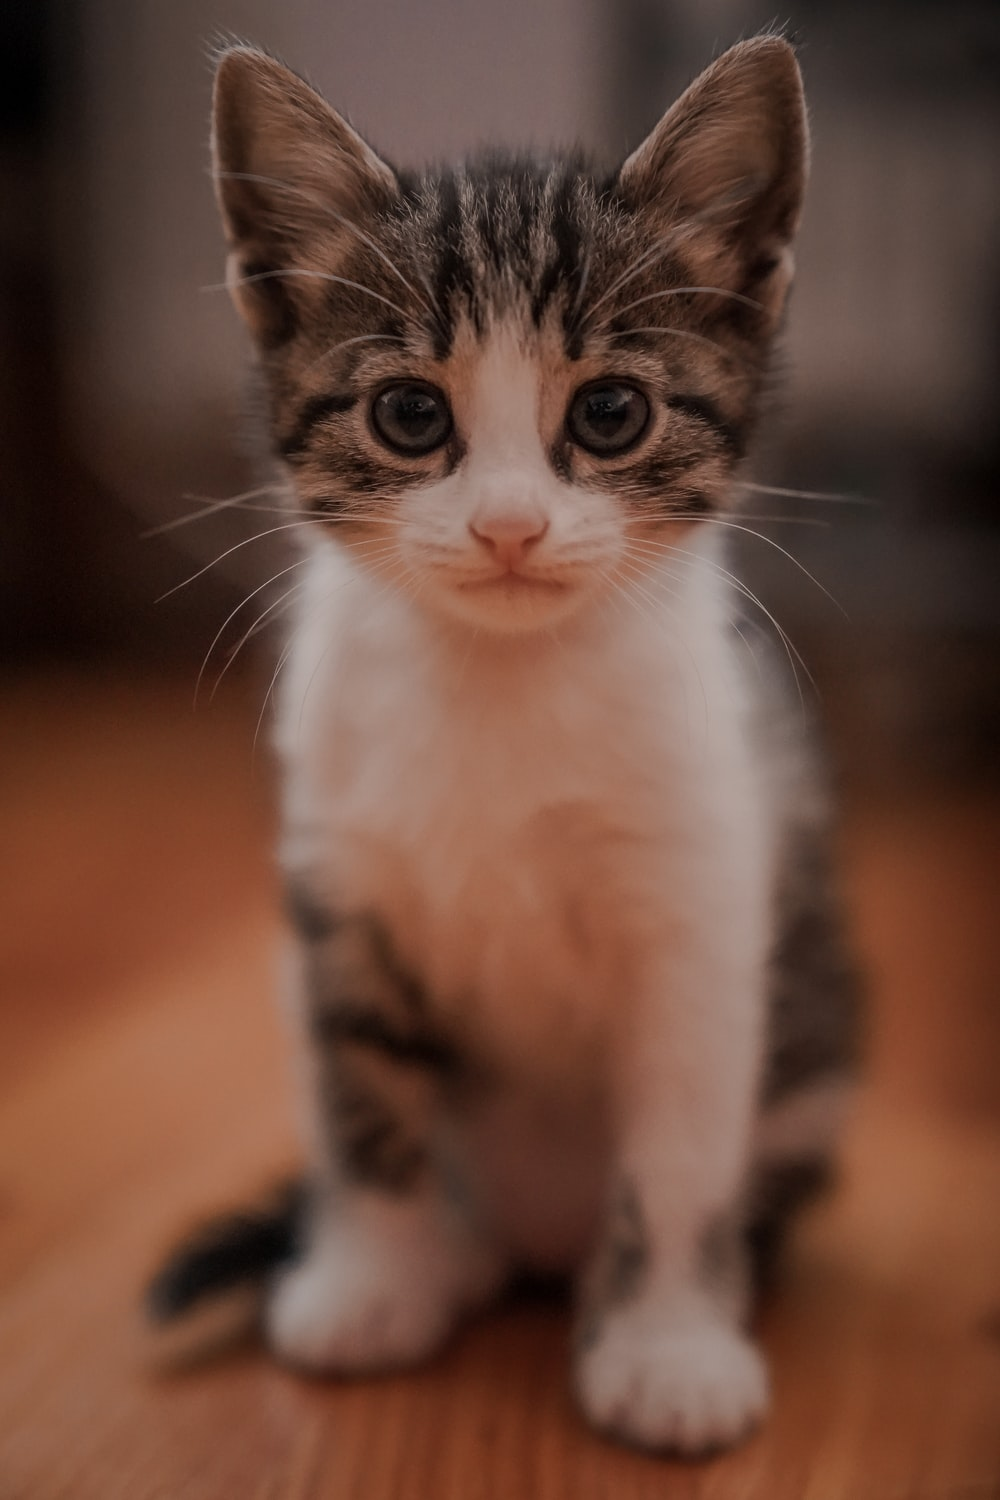
\includegraphics[width=0.3\textwidth]{04-catdog_input_01.jpeg}
	\caption{Masukan pertama sistem eksperimen citra anjing dan kucing}\label{fig:04-catdog-input-01}
\end{figure}

\begin{code}
	\jsoncode{resources/files/tests/catdog_output_01.json}
	\caption{Keluaran pertama sistem eksperimen citra anjing dan kucing}\label{listing:31}
\end{code}

\begin{figure}[H]
    \centering
	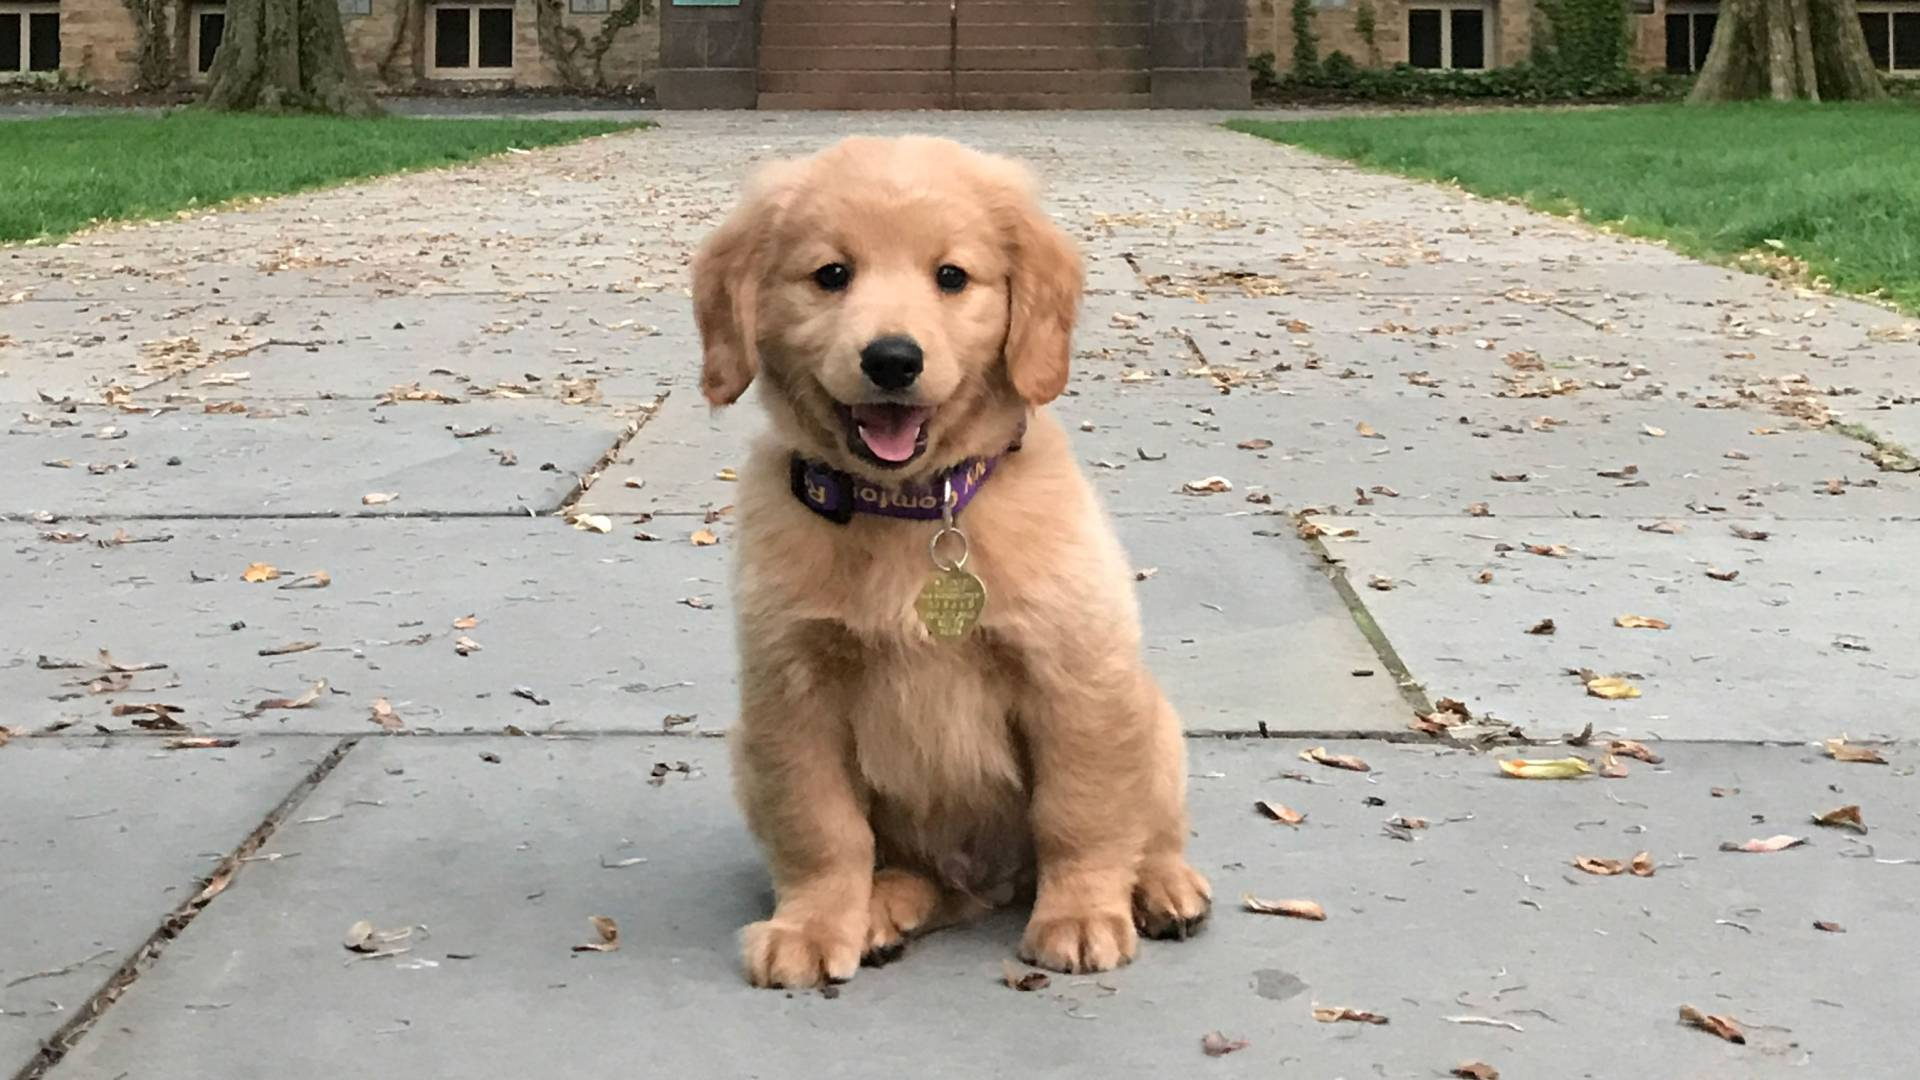
\includegraphics[width=0.3\textwidth]{04-catdog_input_02.jpg}
	\caption{Masukan kedua sistem eksperimen citra anjing dan kucing}\label{fig:04-catdog-input-02}
\end{figure}

\begin{code}
	\jsoncode{resources/files/tests/catdog_output_02.json}
	\caption{Keluaran kedua sistem eksperimen citra anjing dan kucing}\label{listing:32}
\end{code}